\chapter{Introduction}
\label{ch:introduction}

\section{Preface}
Paul Dirac introduced the concept of particles and antiparticles in 1930~\cite{Dirac1930}.
His prediction was based on a purely mathematical argument and explained the negative energy solution of his own relativistic wave equation: the Dirac equation.
The solution he found was a pair of wavefunctions that are each other's complex conjugates.
Three years later, Anderson observed the positron~\cite{Anderson1933}, the electron's complex conjugate.
In 1937, shortly before his mysterious disappearance, the Italian physicist Ettore Majorana found another solution to the Dirac equation, a purely real wavefunction~\cite{Majorana1937}.
The complex conjugate of the real wavefunction is equal to itself, so the particle is its own antiparticle.

Today, many years since the prediction of these Majorana fermions, there is no unambiguous experimental evidence for their existence as a fundamental particle.
However, in condensed matter physics, Majorana fermions have been observed in superconducting materials many years ago~\cite{Kopnin1991}, where they can emerge as (non-fundamental) quasiparticles, more commonly called Bogoliubov quasiparticles.
They are proposed to arise as midgap excitations of a topological superconductor.
In a superconductor, electrons (filled states at energy $E$ above the Fermi level) and holes (unfilled states at $-E$ below the Fermi level) have opposite charges and are each other's complex conjugates.
This charge difference of $2\textrm{e}$ can be absorbed as a Cooper pair in the superconducting condensate.
At the Fermi level ($E=0$, in the middle of the superconducting gap), the eigenstates are charge-neutral superpositions of electrons and holes.
These midgap excitations are called Majorana bound states~\cite{Beenakker2013}.
\footnote{In this thesis we mostly refer to Majorana bound states as Majoranas.}
More about superconductivity and the symmetry that protects the Majoranas in chapter \ref{sec:superconductivity} and \ref{sec:topology}.

In a two-dimensional space, Majorana bound states have non-Abelian exchange statistics~\cite{Stern2010}.
The operation of exchanging two identical particles with such statistics can send the system into a different state with the same particle configuration.
This is different from Abelian exchange statistics (for fermions and bosons), where an exchange can only lead to a global phase shift.
A system with $2N$ Majoranas present is $2^{N}$-fold degenerate, because all decoupled Majoranas are at zero energy.
Interchanging the position of two Majorana bound states (braiding) changes the ground state.
This system is a promising candidate to serve as a quantum bit for topological quantum computation.
Theoretical schemes exist that describe how to perform quantum computation with Majorana bound states in nanowires~\cite{Hyart2013,Alicea2011}, but more about braiding in chapter \ref{sec:braiding}.

Several experimental designs have been proposed to create a topological superconductor and to detect a Majorana bound state~\cite{Kitaev2001,Leijnse2012,Beenakker2013,Alicea2012}.
These proposals consist of superconductors, nanowires, and topological insulators.
A large fraction of the experimental effort~\cite{Mourik2012,Das2012,Deng2012,Churchill2013,Deng2014} is focused on creating Majoranas in semiconducting nanowires with proximity superconductivity, spin-orbit coupling, and magnetic field.
\footnote{This system is introduced in more detail in chapter \ref{sec:MBS}.}
The combination of these effects leads to Majorana bound states at the Fermi energy near the edges of the nanowire~\cite{Oreg2010,Lutchyn2010}.
In 2012 Mourik\textit{ et al}.~observed the signatures of Majorana bound states in a hybrid superconductor semiconductor system~\cite{Mourik2012}.
The theoretical foundation for this platform was initially developed for a single 1D spinful band with intrinsic superconducting pairing~\cite{Lutchyn2010,Oreg2010}.
Due to its compactness, this model can be solved fully analytically, and it predicts that Majorana bound states to appear when $E_{\textrm{Z}}^{2}>\mu^{2}+\Delta^{2}$, so when the Zeeman energy becomes larger than the harmonic mean of the superconducting gap and the chemical potential.

The single-mode model is minimalistic and neglects many physical phenomena that are crucial for understanding the properties of the Majorana bound states.
The existing extensions of this model study multimode wires~\cite{Potter2010a}, better modeling of the induced gap~\cite{Liu2012,Stanescu2014}, the role of electrostatics~\cite{Vuik2016}, disorder~\cite{Potter2012,Pientka2012,Adagideli2014}, and the $k\cdot p$-model~\cite{Stanescu2013a}.
Orbital effect of magnetic field was analyzed in both planar wires~\cite{Osca2015a,Lim2012} and on the surface of a cylinder~\cite{SooLim2013}.

\begin{figure}
\begin{centering}
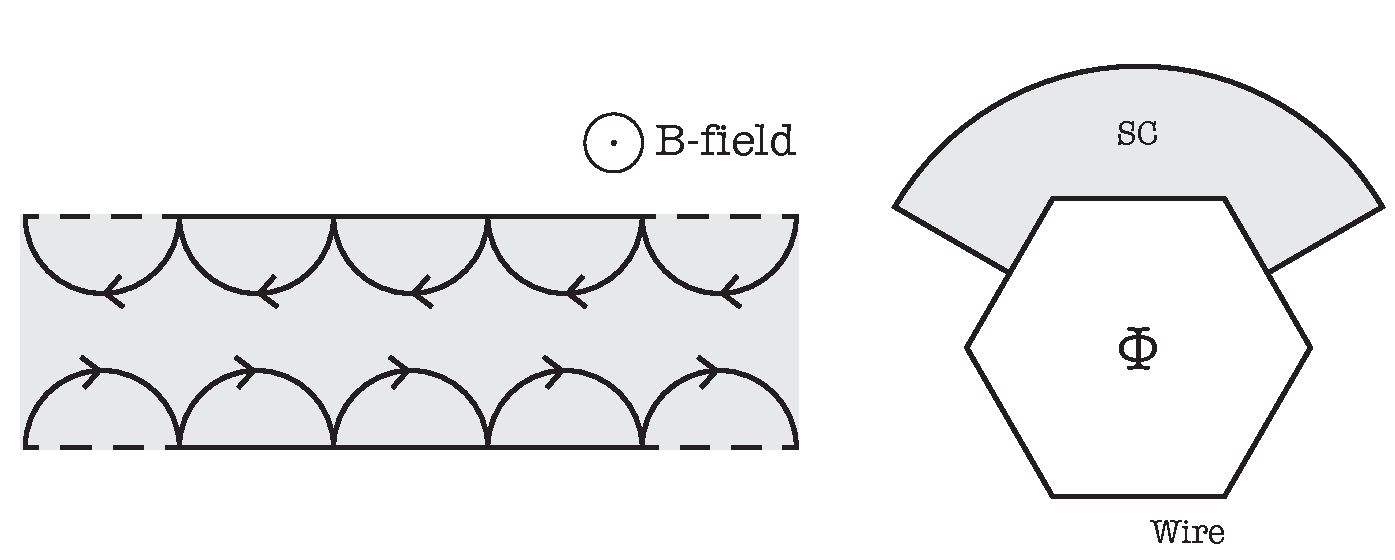
\includegraphics[width=0.95\textwidth]{chapter_introduction/figures/wires.pdf}
\par\end{centering}
\caption{Orbital effect of magnetic field influences the state of particles for both a field parallel and perpendicular to the wire axis.
A perpendicular field induces a skipping orbit motion of the electrons (left).
A magnetic field parallel to the wire shifts the energies due to the effect of magnetic flux $\Phi$.
\label{fig:wire}}
\end{figure}

We systematically study the influence of the orbital effect of the magnetic field on the symmetries of the Hamiltonian and the topological phase diagram for a 3D nanowire, whose specifics are explained in chapter \ref{sec:Model}.
Orbital effect of a magnetic field perpendicular to the wire induces skipping orbit motion of the electrons (see Fig.~\ref{fig:wire}).
The cyclotron radius \footnote{$r_{\textrm{cyclo}}=\frac{mv_{\textrm{F}}}{\textrm{e}B}$, where the Fermi velocity $v_{\textrm{F}}=\sqrt{\frac{2\mu}{m}}$.} becomes comparable to the typical wire diameters $d\sim\SI{100}{nm}$ already at the field of $\SI{0.3}{T}$, and at chemical potential corresponding to the most stable Majoranas.
In addition, a field parallel to the wire shifts the energies of each band due to the effect of magnetic flux.
We expect the shift of the energies to be comparable to the level spacing when the flux through the wire is of an order of a flux quantum.
Our findings are very different from those of Refs.~\cite{Osca2015a,Lim2012,SooLim2013} because we do not limit our analysis to a Hamiltonian with an artificially high spatial symmetry, or low dimensionality.

The theoretical background needed to understand this thesis is introduced in chapter \ref{sec:superconductivity}-\ref{sec:MBS}.
We start with superconductivity and the mean-field approximation that leads to a single particle Hamiltonian that forms the basis of our model.
This Hamiltonian has certain symmetries: this will be the topic of chapter \ref{sec:topology}.
Chapter \ref{sec:braiding} will explain the concept of braiding and will make use of the Majorana properties introduced in the previous chapter.
In chapter \ref{sec:MBS} we proceed to apply this newly learned knowledge to construct a Hamiltonian for a system that can host Majoranas.

\section{\label{sec:superconductivity}Superconductivity}

Superconductivity is a phenomenon that occurs in certain materials when cooled below a characteristic critical temperature $T_{\mathrm{C}}$.
Upon reaching this temperature, the material undergoes a phase transition that results in exactly zero electrical resistance and the expulsion of magnetic fields.
Since the discovery of superconductivity by Heike Kamerlingh Onnes in 1911, considerable efforts have been devoted to finding out how and why it works.
A good understanding of ``conventional'' superconductivity was reached by a pair of remarkable and important theories: the phenomenological Ginzburg-Landau theory and the microscopic BCS theory.
Today research is focused on: exotic superconductors, high $T_{\mathrm{C}}$ superconductors, and hybrid structures consisting of a superconductor and another material.
In this thesis, we study such hybrid structures.

\subsection{BCS theory\label{sec:BCS-theory}}

BCS theory describes superconductivity as a microscopic effect and assumes that two electrons can effectively attract due to electron-phonon coupling and form a Cooper pair.
It postulates that superconductivity is caused by a condensation of Cooper pairs at the Fermi energy\footnote{We assume zero temperature $\left(T=0\right)$, so $E_{\textrm{F}}=\mu$, where $\mu$ is the chemical potential.} $E_{\textrm{F}}$ into a boson-like state, a Bose Einstein condensate.
The model Hamiltonian in the language of second quantization equals~\cite{Gennes1999}

\begin{equation}
\mathcal{H}_{\textrm{BCS}}=\sum_{\bm{k}\sigma}\epsilon_{\bm{k}}c_{\bm{k}\sigma}^{\dagger}c_{\bm{k}\sigma}+\sum_{\bm{k}\bm{l}}V_{\bm{k}\bm{l}}c_{\bm{k}\uparrow}^{\dagger}c_{-\bm{k}\downarrow}^{\dagger}c_{-\bm{l}\downarrow}c_{\bm{l}\uparrow},\label{eq:BCS}
\end{equation}

where

\begin{tabular}{ll}
 $c$  & annihilation operator electron \tabularnewline
 $c^{\dagger}$ & creation operator electron\tabularnewline
 $\epsilon_{k}$  &  $E_{k}-\mu$\tabularnewline
$\mu$ & chemical potential\tabularnewline
$E_{k}$ & kinetic energy ($\frac{\hbar^{2}k^{2}}{2m}$)\tabularnewline
$m$ & mass\tabularnewline
 $k$  & momentum\tabularnewline
 $\sigma,\uparrow,\downarrow$  & spin of electron\tabularnewline
 $V_{\bm{kl}}$ & interaction potential.\tabularnewline
\end{tabular}


The interaction term includes only the Cooper pairs, which consist of two electrons with opposite spin (s-wave symmetry) and opposite momentum and can be denoted as $(\bm{\bm{k}}\uparrow,-\bm{k}\uparrow)$.
Finding the ground state of this so-called pairing Hamiltonian is impossible; therefore, we have to make an approximation.
A classic approximation scheme that describes the behavior of conventional superconductors remarkably well is the mean-field approximation.
First we define the quantity
\[
b_{\bm{k}}=\left\langle c_{\bm{k}\uparrow}c_{-\bm{k}\downarrow}\right\rangle ,
\]
which we use to define the so-called gap energy
\[
\Delta_{\bm{k}}=-\sum_{\bm{k'}}V_{\bm{kk'}}b_{\bm{k'}}.
\]
We write $c_{\bm{k}\uparrow}^{\dagger}c_{-\bm{k}\downarrow}^{\dagger}c_{-\bm{l}\downarrow}c_{\bm{l}\uparrow}$ from Eq.~\ref{eq:BCS} as

\begin{equation}
c_{\bm{k}\uparrow}^{\dagger}c_{-\bm{k}\downarrow}^{\dagger}c_{-\bm{l}\downarrow}c_{\bm{l}\uparrow}=\left(c_{\bm{k}\uparrow}^{\dagger}c_{-\bm{k}\downarrow}^{\dagger}-b_{\bm{k}}^{\dagger}+b_{\bm{k}}^{\dagger}\right)\left(c_{-\bm{l}\downarrow}c_{\bm{l}\uparrow}-b_{\bm{l}}+b_{\bm{l}}\right),\label{eq:MF}
\end{equation}
and expand the products.
Neglecting the second-order fluctuation term  $\left(c_{\bm{k}\uparrow}^{\dagger}c_{-\bm{k}\downarrow}^{\dagger}-b_{\bm{k}}^{\dagger}\right)\left(c_{-\bm{l}\downarrow}c_{\bm{l}\uparrow}-b_{\bm{k}}\right)$ in Eq.~\ref{eq:MF} and using it to rewrite Eq.~\ref{eq:BCS} gives
\begin{equation}
\mathcal{H}_{\textrm{BCS}_{\textrm{MF}}}=\underset{\bm{k},\sigma}{\sum}\epsilon_{\bm{k}}c_{\bm{k}\sigma}^{\dagger}c_{\bm{k}\sigma}-\underset{\bm{k}}{\sum}\left(\Delta_{\bm{k}}c_{\bm{k}\uparrow}^{\dagger}c_{-\bm{k}\downarrow}^{\dagger}+\Delta_{\bm{k}}^{*}c_{-\bm{k}\downarrow}c_{\bm{k}\uparrow}-\Delta_{\bm{k}}b_{\bm{k}}^{*}\right),\label{eq:BCS_MF}
\end{equation}
where the last term is just a constant that can be neglected.
We now introduce Nambu spinors
\begin{equation}
\Psi_{\bm{k}}=\left(\begin{array}{c}
c_{\bm{k}\uparrow}\\
c_{-\bm{k}\downarrow}^{\dagger}
\end{array}\right)\label{eq:Nambu}
\end{equation}
and write Eq.~\ref{eq:BCS_MF} in matrix representation
\[
\mathcal{H}_{\textrm{BCS}_{\textrm{MF}}}=\underset{\bm{k}}{\sum}\Psi_{\bm{k}}^{\dagger}\underset{H_{\textrm{BdG}}}{\underbrace{\left(\begin{array}{cc}
\epsilon_{\bm{k}} & \Delta\\
\Delta_{\bm{k}}^{*} & -\epsilon_{\bm{k}}
\end{array}\right)}}\Psi_{\bm{k}}.
\]
We can diagonalize the Bogoliubov-de Gennes Hamiltonian $H_{\textrm{BdG}}$ using the unitary Boguliubov transformation matrix $U_{\textrm{B}}$ and solve the eigenvalue problem.
Alternatively, we can square $H_{\textrm{BdG}}$ which gives a diagonal matrix
\[
H_{\textrm{BdG}}^{2}=\left(\begin{array}{cc}
\epsilon_{\bm{k}}^{2}+\left|\Delta\right|^{2} & 0\\
0 & \epsilon_{\bm{k}}^{2}+\left|\Delta\right|^{2}
\end{array}\right)
\]
where we can use that the eigenvalues are the square root of the eigenvalues of $H_{\textrm{BdG}}$.
This immediately result in the spectrum
\begin{equation}
E=\pm\sqrt{\epsilon_{\bm{k}}^{2}+\left|\Delta\right|^{2}}.\label{eq:SC_spectrum}
\end{equation}

The Bogoliubov-de Gennes Hamiltonian acts on the Nambu spinors (Eq.~\ref{eq:Nambu}) whose first half is composed out of annihilation operators of electrons, and the second half out of creations operators of the same electrons.
In order to go to first quantization, we can see the latter creation operators as annihilation operators of an extra set of holes and thereby double the number of degrees of freedom in the system.

Besides the Pauli matrices that act on spin ($\sigma_{i}$ where $i\in x,y,z$) we introduce $\tau_{i}$ to act on the electron-hole degree of freedom.
The Hamiltonian becomes a $4\times4$ matrix\footnote{Here $\otimes$ denotes the Kronecker product and we usually omit $\sigma_{0}$ and $\tau_{0}$.}
\[
H_{\textrm{BdG}}=\epsilon_{k}\tau_{z}\otimes\sigma_{0}+\Delta\tau_{x}\otimes\sigma_{0}=\left(\begin{array}{cccc}
\epsilon_{k} & 0 & \Delta & 0\\
0 & \epsilon_{k} & 0 & \Delta\\
\Delta & 0 & -\epsilon_{k} & 0\\
0 & \Delta & 0 & -\epsilon_{k}
\end{array}\right)
\]
which acts on the wavefunction
\begin{equation}
\Psi=\left(\psi_{\textrm{e}\uparrow},\psi_{\textrm{e}\downarrow},\psi_{\textrm{h}\downarrow},-\psi_{\textrm{h}\uparrow}\right)^{T},\label{eq:4wf}
\end{equation}
where $\psi_{\textrm{e}}$, $\psi_{\textrm{h}}$ are the electron and hole components of the wave function, and $\psi_{\uparrow}$, $\psi_{\downarrow}$ are the spin-up and spin-down states.
Now $H_{\textrm{BdG}}$ has an additional symmetry because the holes are related to the electrons.
Symmetry will be the topic of the next chapter.


\section{\label{sec:topology}Topology and symmetry}

The concept of symmetry plays a fundamental part in physics.
For a physical system it is a very important characteristic that in many cases has a decisive effect on the behavior of the system.
For example, Noether's theorem states that each continuous symmetry of a physical system implies that a certain physical property of that system is conserved.
In condensed matter systems only three discrete symmetries are important: time-reversal symmetry $\mathcal{T}$, particle-hole symmetry $\mathcal{P}$, and chiral symmetry $\mathcal{C}$.
Wigner's theorem states that a symmetry must either be a unitary or an anti-unitary operator.
Both $\mathcal{T}$ and $\mathcal{P}$ have anti-unitary operators and may square either to $+1$ or $-1$ depending on the specifics of the system.
Chiral symmetries have a unitary operator and always squares to $+1$.
Together these three symmetries form ten symmetry classes~\cite{Altland1997}, each class characterized by the type and absence or presence of these symmetries.

Topology studies whether objects can be continuously transformed into each other.
The object that is studied in condensed matter is the Hamiltonian of a system.
If two Hamiltonians can be continuously transformed\footnote{An example of a continuous transformation from $H_{1}$ to $H_{2}$: $H=\alpha H_{1}+(1-\alpha)H_{2}$ where $\alpha=0\rightarrow1$.} into each other without changing the topological invariant: the systems are said to be topologically equivalent.
The dimensionality and symmetry class determine the type of topological invariant of a system.
For example, such a topological invariant of the system we study in this thesis indicates the presence or absence of Majoranas.

\subsection{Particle-hole symmetry\label{sec:phs}}

Mathematically a particle-hole symmetry $\mathcal{P}$ is expressed as an operator that is anti-unitary and anti-commutes with the Hamiltonian.
An example of where this symmetry manifests, is the Bogoliubov-de Gennes Hamiltonian $H_{\textrm{BdG}}$ introduced in section \ref{sec:BCS-theory}.
Here, $H_{\textrm{BdG}}$ acts on a two-component wave function $\psi_{\textrm{BdG}}=\left(u,v\right)^{T}$ with $u$ electron component and $v$ the hole component.
The symmetry of this Hamiltonian is most obvious from its dispersion relation, where each eigenstate $\psi_{E}=\left(u_{0},v_{0}\right)^{T}$ has a particle-hole symmetric partner at $\psi_{-E}=\left(\mathcal{P}u_{0},\mathcal{P}v_{0}\right)^{T}$.
In constructing $H_{\textrm{BdG}}$, we artificially doubled the degrees of freedom by considering electrons and holes separately.
Therefore, the creation operator $c^{\dagger}$ of the quasiparticle in the $\psi_{E}$ state is equal to the annihilation operator $c$ of the quasiparticle in the $\psi_{-E}$ state.
It is then clear that $\psi_{E}$ and $\psi_{-E}$ correspond to the same quasiparticle, and the creation of a quasiparticle with positive energy is identical to the annihilation of a quasiparticle with negative energy.

At zero energy, something curious happens: here we have a state $\psi_{0}$ that upon applying $\mathcal{P}$ is transformed into itself $\mathcal{P}\psi_{0}=\psi_{0}$.
This state has a creation operator $\gamma^{\dagger}$ that is identical to the annihilation operator $\gamma$ of itself, so $\gamma^{\dagger}=\gamma$.
We call this property the Majorana condition, and operators that satisfy this property are called Majorana fermions.
If we use the Majorana condition in the fermionic commutation relation
\[
\gamma^{\dagger}\gamma+\gamma\gamma^{\dagger}=1
\]
we get $\gamma^{\dagger}\gamma=1/2$ and see that the Majorana state is always half occupied.
Removing a Majorana from zero energy is, therefore, only possible if it is paired with another Majorana to form a fermionic mode, but more about Majoranas in chapter \ref{sec:braiding}.

In a one or higher dimensional system, the operator $\mathcal{P}$ will not only send $E\rightarrow-E$ but will also send the momentum $k\rightarrow-k$ as
\[
\mathcal{P^{\dagger}}H\left(k\right)\mathcal{P}=-H\left(-k\right),
\]
because $\mathcal{P}$ is an anti-unitary operator.

\subsection{Chiral symmetry\label{sec:Chiral-symmetry}}

A chiral symmetry $\mathcal{C}$ is expressed as an operator that is unitary and anti-commutes with the Hamiltonian.
A system where the lattice has two sublattices, such as the hexagonal lattice of graphene, can have a chiral symmetry if we only consider the first neighbor hopping.
If we split all the degrees of freedom into two groups (say group A and group B) the Hamiltonian can be written as
\[
H=\begin{pmatrix}0 & H_{AB}\\
H_{AB}^{\dagger} & 0
\end{pmatrix}.
\]
Here the unitary Pauli matrix $\sigma_{z}$ anti-commutes with the Hamiltonian and, therefore, is a chiral symmetry.
We can apply this chiral symmetry to the Hamiltonian as
\[
\sigma_{z}H\sigma_{z}=-H,
\]
and see that this operation makes the spectrum symmetric with respect to zero energy.
Unlike particle-hole symmetry, $\mathcal{C}$ will leave momentum untouched as
\[
\mathcal{C^{\dagger}}H\left(k\right)\mathcal{C}=-H\left(k\right),
\]
because of its unitarity property.

\subsection{Topology}

As mentioned in the introduction, the dimensionality and symmetry class determine the type of topological invariant of a system.
In this thesis, we study a system that is fundamentally of symmetry class $\mathcal{D}$; this is because the Hamiltonian has a particle-hole symmetry that squares to $+1$.  % XXX: NOT TRUE
The zero-dimensional topological invariant of symmetry class D is the sign of the Pfaffian of the Hamiltonian: $\sgn\Pf\left(H\right)$, which can only assume two values, $+1$ or $-1$.
The Pfaffian for an anti-symmetric matrix is related to the determinant as $\Pf(A)^{2}=\det(A)$.
However, in many cases, the Hamiltonian is not anti-symmetric; fortunately, we can always perform a basis transformation on a particle-hole symmetric Hamiltonian that makes it so.

We still did not mention the physical reason for why a topological invariant would change.
The topological invariant is only defined for a system with an energy gap, which means the Hamiltonian of the system has no eigenvalues in a finite interval around zero energy.
If we can continuously transform a Hamiltonian $H_{1}$ into another Hamiltonian $H_{2}$ without ever closing the energy gap, we say $H_{1}$ and $H_{2}$ are topologically equivalent, and thus have the same topological invariant.


\section{\label{sec:braiding}Braiding}

For many researchers that work on Majoranas, the ultimate motivation to study them is the fact that they have a fascinating property, non-Abelian quantum statistics.
Quantum statistic studies what happens to wavefunctions describing identical particles when their positions are exchanged in space.
In our quantum mechanics courses, we learned that particles are divided into two classes according to quantum statistics: bosons which stay the same under the exchange and fermions for which the wavefunction changes sign.
However, Majorana bound states do not belong to either of these.
The operation of exchanging two Majoranas can send the system into a different state with the same particle configuration.
Explaining how one could experimentally perform a braiding operation is beyond the scope of this thesis; therefore, we will focus on the mathematical operations that describe the braiding process.

Exchanging two Majoranas in 1D is ill-defined because it is impossible to swap them without having them collide, which would annihilate them.
We can construct a network of nanowires to form T-junctions (see Fig.~\ref{fig:Majorana-T-junction}), which allows us to exchange positions of Majoranas.
Here, one can temporarily move a Majorana to one of the unoccupied wires and perform the exchange without the Majoranas ever becoming too close to each other.

\begin{figure}
\begin{centering}
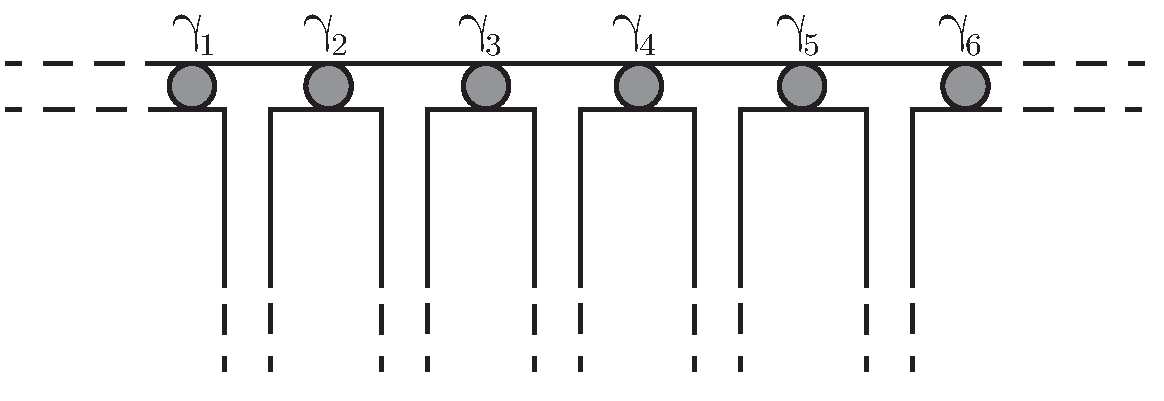
\includegraphics[width=0.95\textwidth]{chapter_introduction/figures/T-junction-network.pdf}
\par\end{centering}
\centering{}
\caption{Majorana T-junction.
The circles represent the Majoranas $\gamma_{1}...\gamma_{6}$.
This network of nanowires allows for the exchange of two Majoranas without having them collide.
This is possible by temporarily bringing a Majorana to one of the
vertical wires and then swapping the position of the other Majorana.
\label{fig:Majorana-T-junction}}
\end{figure}

The only thing that distinguishes Majoranas is their position in the network.
That means that if we exchanged two Majoranas in space, the system would look exactly the same as it looked before the exchange.
We now assume the energy spectrum is gapped for $0<E<\Delta$ with the Majorana ground state at $E=0$.
If this ground state contains several Majoranas, there will be several states all at zero energy, forming a \textquotedblleft ground state manifold\textquotedblright .
From now on we only consider the states corresponding to the Majoranas and neglect the states that live in the bulk ( $E\geq\Delta$).\\ As mentioned in chapter \ref{sec:phs}, a Majorana has only half a degree of freedom and thus, they can only be assigned quantum states in pairs.
In Fig.~\ref{fig:Majorana-T-junction} we see six Majoranas (3 pairs), but for generality lets consider $N$ pairs.
By pairing two Majoranas (two times half a degree of freedom), we can form fermionic modes that will give us two possible degenerate quantum states, either unoccupied $\ket0$ or occupied $\ket1$.
By pairing up neighboring Majoranas\foreignlanguage{english}{ $\gamma_{2n-1}$} and \foreignlanguage{english}{$\gamma_{2n}$} we get a creation operator that is its own complex conjugate $c_{n}^{\dagger}=\tfrac{1}{2}(\gamma_{2n-1}+i\gamma_{2n})$, where $c$ is a fermionic creation operator.
Each pair gives two possible quantum states, so $N$ pairs will have $2^{N}$ possible states.
We can represent every such state with a ket
\[
\left|s_{1},s_{2},\dots,s_{N}\right\rangle ,
\]
where $s_{n}$ is either unoccupied $0$ or occupied $1$.
These states form a complete basis of the Hilbert space of the set of Majoranas.

We define the fermion parity operator
\[
P_{n}\equiv1-2c_{n}^{\dagger}c_{n}=i\gamma_{2n-1}\gamma_{2n},
\]
that acts on the states and where we recognize the $c_{n}^{\dagger}c_{n}$ term as the number operator.
All basis states in the Hilbert space of Majoranas are eigenstates of $P_{n}$.
For example, we have
\[
P_{1}\left|0,\dots\right\rangle \ =(1-2c_{1}^{\dagger}c_{1})\left|0,\dots\right\rangle =+\left|0,\dots\right\rangle ,
\]

\[
P_{1}\left|1,\dots\right\rangle \ =(1-2c_{1}^{\dagger}c_{1})\left|1,\dots\right\rangle =-\left|1,\dots\right\rangle .
\]

Another essential property of Majoranas is that a pair of Majorana operators all anti-commute with each other.
So
\[
(\gamma_{1}\gamma_{2})(\gamma_{3}\gamma_{4})=(\gamma_{3}\gamma_{4})(\gamma_{1}\gamma_{2}),
\]
but when the pairs share a Majorana they do not commute anymore
\[
(\gamma_{1}\gamma_{2})(\gamma_{2}\gamma_{3})=-(\gamma_{2}\gamma_{3})(\gamma_{1}\gamma_{2}).
\]

In chapter \ref{sec:superconductivity} you might have noticed that the total particle number in the Hamiltonian is not conserved; however, the parity is conserved.
The total parity can be obtained by multiplying all parity operators
\[
P_{\textrm{tot}}=P_{1}\cdot P_{2}\cdot\,\dots\,\cdot P_{N}=i^{N}\gamma_{1}\gamma_{2}\dots\gamma_{2N}.
\]
where $P_{\textrm{tot}}$ has eigenvalues $\pm1$.
The parity is an observable and can, therefore, be experimentally measured.


We can now start to think about what would happen when we exchange two Majoranas~\cite{Ivanov2001}.
Our ground state manifold $\ket\Psi$ will never leave the ground state if we perform the exchange slowly enough.
The exchange of two Majoranas $\gamma_{n}$ and $\gamma_{m}$ will change the ground state $\left|\Psi\right\rangle \to U\left|\Psi\right\rangle $ where $U$ is a unitary operator.
The exact form of $U$ can be derived without a direct calculation.
We do this by assuming that $U$ only depends on the Majoranas involved in the exchange ( $\gamma_{n}$ and $\gamma_{m}$) and by using that the slow exchange does not change the parity of the system because the system stays gapped at all times.
Since the parity is conserved we know: $U$ commutes with the total fermion parity $[U,P_{\textrm{tot}}]=0$, and that $U$ can only depend on the product $i\gamma_{n}\gamma_{m}$.
This product is Hermitian, so we can create a unitary operator by taking the exponential of $i$ times this Hermitian operator as
\[
U\equiv\exp(\beta\gamma_{n}\gamma_{m})=\cos(\beta)+\gamma_{n}\gamma_{m}\sin(\beta),
\]
where $\beta$ is a real coefficient to be determined.
In the last equality we used $(\gamma_{n}\gamma_{m})^{2}=\gamma_{n}\gamma_{m}\gamma_{n}\gamma_{m}=-\gamma_{n}\underset{=1}{\underbrace{\gamma_{m}\gamma_{m}}}\gamma_{n}=-1$
in the Taylor expansion.


We now move to the Heisenberg picture where we look at the evolution of the Majorana operators in time
\[
\gamma_{n}\to U\gamma_{n}U^{\dagger}=\left(\cos\beta+\gamma_{n}\gamma_{m}\sin\beta\right)\gamma_{n}\left(\cos\beta+\gamma_{m}^{\dagger}\gamma_{n}^{\dagger}\sin\beta\right)
\]

\[
=\gamma_{n}\cos^{2}\beta+\left(\gamma_{n}\gamma_{m}^{\dagger}\gamma_{n}^{\dagger}+\gamma_{n}\gamma_{m}\gamma_{n}\right)\sin\beta\cos\beta+\gamma_{n}\gamma_{m}\gamma_{n}\gamma_{m}^{\dagger}\gamma_{n}^{\dagger}\sin^{2}\beta
\]

\[
=\gamma_{n}\cos^{2}\beta-\gamma_{n}^{\dagger}\sin^{2}\beta-2\gamma_{m}\sin\beta\cos\beta
\]

\[
=\gamma_{n}\cos2\beta-\gamma_{m}\sin2\beta
\]
Similarly we get
\[
\gamma_{m}\to U\gamma_{m}U^{\dagger}=\gamma_{m}\cos2\beta+\gamma_{n}\sin2\beta.
\]
After the exchange happened we know that $\gamma_{m}\to\gamma_{n}$ and $\gamma_{n}\to\gamma_{m}$, this leads to $\beta=\pm\pi/4$.
The two signs make sense; this distinguishes the clockwise and the counterclockwise exchange of the Majoranas.
We now found an operator that exchanges two Majoranas
\begin{equation}
U=\exp\left(\pm\frac{\pi}{4}\gamma_{n}\gamma_{m}\right)=\tfrac{1}{\sqrt{2}}\left(1\pm\gamma_{n}\gamma_{m}\right).\label{eq:U_nm}
\end{equation}

As an example, lets now look at what happens when we have just four Majoranas $\gamma_{1}$, $\gamma_{2}$, $\gamma_{3}$ and $\gamma_{4}$.
The four basis states in the ground state manifold are
\begin{equation}
\left|00\right\rangle ,\left|01\right\rangle ,\left|10\right\rangle ,\left|11\right\rangle ,\label{eq:basis}
\end{equation}
where the first number is the occupation number of the fermionic mode $c_{1}^{\dagger}=\tfrac{1}{2}(\gamma_{1}+i\gamma_{2})$ and the second number the occupation number of $c_{2}^{\dagger}=\tfrac{1}{2}(\gamma_{3}+i\gamma_{4})$.
For instance, if we start from the state $\left|00\right\rangle $ and we exchange $\gamma_{2}$ and $\gamma_{3}$ by applying $U_{23}=\tfrac{1}{\sqrt{2}}\left(1\pm\gamma_{2}\gamma_{3}\right)$, we obtain\footnote{See appendix \ref{chap:U_der} for derivations of $U_{nm}$.}
\[
\left|00\right\rangle \to U_{23}\left|00\right\rangle =\tfrac{1}{\sqrt{2}}\left(\left|00\right\rangle +i\left|11\right\rangle \right).
\]
Here we see a superposition of states, which is not like bosons or fermions at all, where the exchange can only change the sign.
This property makes Majoranas non-Abelian anyons, and the exchange of two non-Abelian anyons is usually called braiding.



\section{\label{sec:MBS}Creating Majoranas in a nanowire}

The combined effect of superconductivity, spin-orbit coupling, and a Zeeman field can lead to the appearance of Majoranas near the edges of the wire~\cite{Lutchyn2010,Oreg2010}.
Before we can understand why this might happen, we will study the effects of the various terms in the Hamiltonian.
The appearance of Majoranas is a topological effect and is accompanied by the change of the topological invariant $Q$ of symmetry class D.
As discussed in chapter \ref{sec:topology}, this invariant can only assume $Q=+1$ (no Majoranas) and $Q=-1$ (Majoranas present) and changes when the bandgap is closed.


\begin{figure}
\begin{centering}
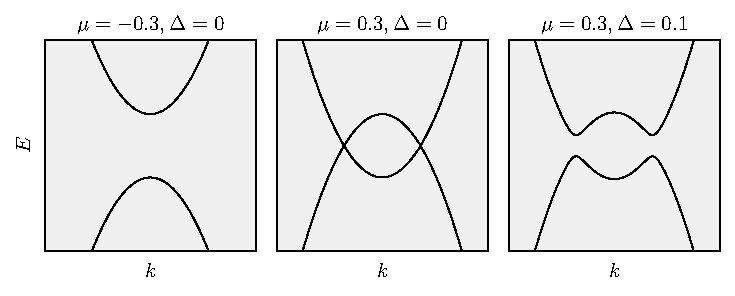
\includegraphics[width=0.95\textwidth]{chapter_introduction/figures/triv_topo_bandstructure.pdf}
\par\end{centering}
\caption{Band structures of Hamiltonians with chemical potential $\mu=-0.3$
and superconducting gap $\Delta=0$ (left); $\mu=0.3$ and $\Delta=0$
(middle); $\mu=0.3$, $\Delta=0.1$.
\label{fig:triv_topo_bandstructure}}
\end{figure}

The complete model Hamiltonian is rather complicated; we will, therefore, start with a one-dimensional single band Hamiltonian in its simplest form and study the band structures while adding terms needed to make a topological band structure and ``engineer'' our way towards Majoranas.
The Hamiltonian in its simplest form is quadratic in momentum and has an off-set in chemical potential $\mu$  \begin{equation}
H=\left(\frac{\bm{p}^{2}}{2m}-\mu\right)\tau_{z},\label{eq:simple_ham}
\end{equation}
where $\tau_{z}$ is a Pauli matrix that acts on the electron-hole substructure.
The band structure for this Hamiltonian with $\mu=-0.3$ is shown in Fig.~\ref{fig:triv_topo_bandstructure} (left).
We now assume that this band structure is topologically trivial and has $Q=+1$.
The wavefunction where we doubled the degrees of freedom has four components (Eq.~\ref{eq:4wf}).
Therefore, the bands in Fig.~\ref{fig:triv_topo_bandstructure} (left) are doubly degenerate because both spin up and down is on the same energy.
The $\tau_{z}$ in the Hamiltonian ensures that the electrons are at positive energy $E$ and the holes on $-E$.


The next step is to create a bandgap closure in order to change $Q$.
This is done by raising $\mu$, which shifts the bands, see Fig.~\ref{fig:triv_topo_bandstructure} (middle).
In chapter \ref{sec:topology}, we explained that the topological invariant is only defined for a system with an energy gap.
This band structure has no bandgap, so it cannot be topological.
Further, in chapter \ref{sec:superconductivity} we saw that having a superconductor leads to a gapped spectrum (Eq.~\ref{eq:SC_spectrum}), so adding $\Delta\tau_{x}$ (which results in the the Bogoliubov-de Gennes Hamiltonian)
\[
H_{\textrm{BdG}}=\left(\frac{\bm{p}^{2}}{2m}-\mu\right)\tau_{z}+\Delta\tau_{x},
\]
creates a gap because $\tau_{x}$ mixes the electron and holes (see Fig.~\ref{fig:triv_topo_bandstructure} (right)).
We can now argue that Fig.~\ref{fig:triv_topo_bandstructure} (right) is a topological band structure because the bandgap closed and consequently: $Q$ changed.
However, $Q$ changed twice, because the doubly degenerate spin bands both crossed zero energy simultaneously, and therefore we need some more terms to reach our goal.

\subsection{Zeeman splitting}

We are now left in a state where for every eigenstate, there is at least one more eigenstate with the same energy, this is called Kramer's degeneracy, and it needs to be broken in order to make Majoranas.
\footnote{With Kramer's degeneracy, we would make two Majoranas per edge.}
To couple to spin we introduce the Zeeman field in the Hamiltonian, which now becomes
\begin{equation}
H_{\textrm{BdG}}=\left(\frac{\bm{p}^{2}}{2m}-\mu\right)\tau_{z}+\Delta\tau_{x}+\frac{1}{2}g\mu_{\textrm{B}}B\sigma_{x},\label{eq:zeeman}
\end{equation}
where $g$ is the Landé factor, $\mu_{\textrm{B}}$ the Bohr magneton and $B$ magnetic field along $x$, parallel to the wire direction.
In Fig.~\ref{fig:zeeman} band structures are plotted for different values of magnetic field.

\begin{figure}
\begin{centering}
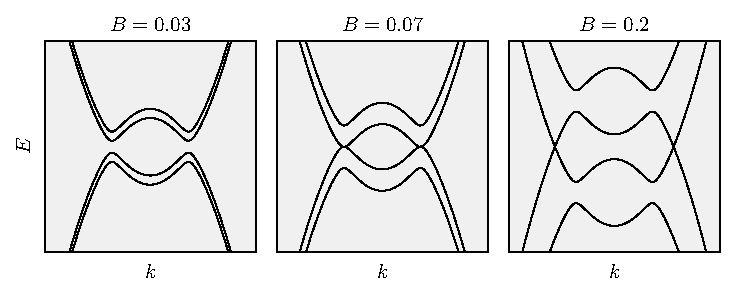
\includegraphics[width=0.95\textwidth]{chapter_introduction/figures/zeeman.pdf}
\par\end{centering}
\caption{Band structures of Eq.~\ref{eq:zeeman} for different values of magnetic field and $\Delta=0.1$, $\mu=0.3$.
\label{fig:zeeman}}
\end{figure}
We see that the Kramer's degeneracy is broken when we turn on the magnetic field, because there are no different states with the same energy anymore.
The bands that move towards each other have opposite spin (orthogonal states), and as we see in Fig.~\ref{fig:zeeman} (middle and left), these spins do not couple.
The problem is that Zeeman conserves spin in $x$-direction, and therefore spin is still a good quantum number.
We know that Majoranas must be spinless because they are their own complex conjugate.


\subsection{Spin-orbit coupling}

The solution to this last problem is spin-orbit coupling, which in its simplest form is Rashba: $H_{\textrm{Rashba}}=-\alpha p_{x}\sigma_{y}\tau_{z}$.
The Hamiltonian is now complete and equals
\begin{equation}
H_{\textrm{BdG}}=\left(\frac{\bm{p}^{2}}{2m}-\mu\right)\tau_{z}+\Delta\tau_{x}+\frac{1}{2}g\mu_{\textrm{B}}B\sigma_{x}-\alpha p_{x}\sigma_{y}\tau_{z}.\label{eq:rashba}
\end{equation}
Lets first see why spin-orbit by itself---because is seems to couple spin---is not sufficient to break the Kramer's degeneracy and why we needed the Zeeman term in the first place.
In Fig.~\ref{fig:SO_no_zeeman} we see that upon raising $\alpha$ the different spin bands move away in either $+k$ or $-k$ direction.
However, Kramer's degeneracy is not broken because there are two states with the same energy at $k=0$.

\begin{figure}
\centering{}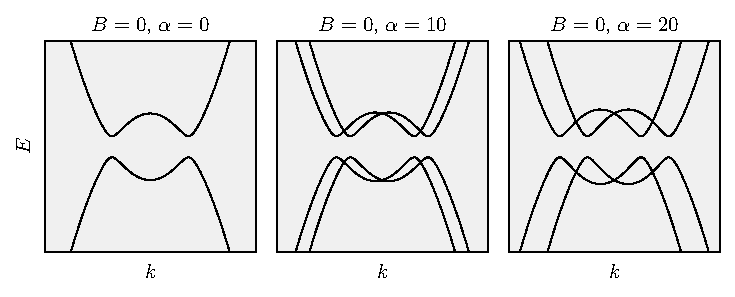
\includegraphics[width=0.95\textwidth]{chapter_introduction/figures/SO_no_zeeman.pdf}
\caption{Band structures of Eq.~\ref{eq:rashba} for different values of spin-orbit coupling $\alpha$ and $B=0$, $\Delta=0.1$, $\mu=0.3$.
\label{fig:SO_no_zeeman}}
\end{figure}
If we now also turn on magnetic field we see that spin-orbit opens the gap at finite $k$ (see Fig.~\ref{fig:SO_and_zeeman}).
This system will accommodate Majoranas at $E=0$ and is called topologically nontrivial, for it has no degeneracies, a gapped spectrum, and $Q=-1$.

\begin{figure}
\centering{}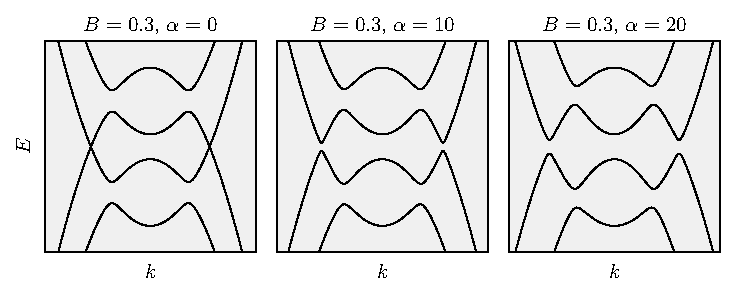
\includegraphics[width=0.95\textwidth]{chapter_introduction/figures/SO_and_zeeman.pdf}
\caption{Band structures of Eq.~\ref{eq:rashba} for different values of spin-orbit coupling $\alpha$ and $B=0.3$, $\Delta=0.1$, $\mu=0.3$.
\label{fig:SO_and_zeeman}}
\end{figure}


\subsection{Wavefunctions}

With a topological band structure, we expect Majoranas to appear near
the edges of the nanowires.
We can check if this happens by calculating the wavefunctions of a finite wire and plotting the probability density of the wavefunction corresponding to the lowest energy.
In Fig.~\ref{fig:wavefunction_1d} (left), we see the probability density of the lowest energy mode (the Majorana wavefunction) is indeed localized near edges of the nanowire.
The wavefunction decays exponentially with decay length $\xi$.

\begin{figure}
\begin{centering}
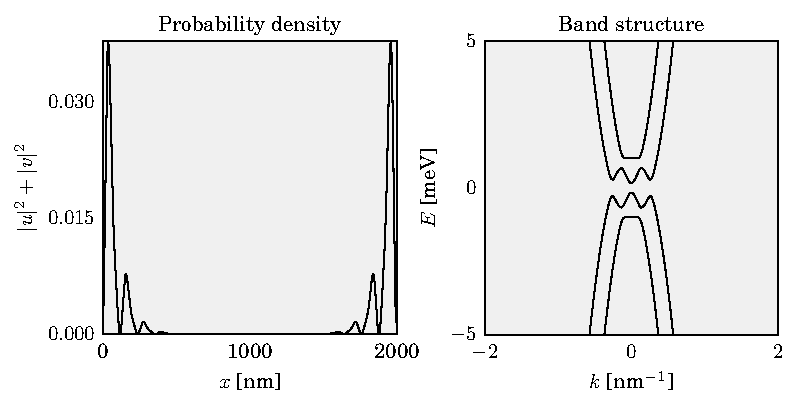
\includegraphics[width=0.95\textwidth]{chapter_introduction/figures/wavefunction_1d.pdf}
\par\end{centering}
\caption{Probability density and band structure of a 1D system.
The probability density of the lowest energy wavefunction (Majorana wavefunction) of a \SI{2}{\micro\metre} long nanowire (left) and a topological band structure (right) with the same parameter values, but for an infinite system.
The Majorana length $\xi$---the decay length of the wavefunction---in
the left plot is $\xi=\SI{315}{nm}$.
\label{fig:wavefunction_1d}}
\end{figure}

In 2D the model Hamiltonian (Eq.~\ref{eq:rashba}) looks very similar
\begin{equation}
H_{\textrm{BdG}}=\left(\frac{\bm{p}^{2}}{2m}-\mu\right)\tau_{z}+\Delta\tau_{x}+\frac{1}{2}g\mu_{\textrm{B}}B\sigma_{x}+\alpha\left(p_{y}\sigma_{x}-p_{x}\sigma_{y}\right)\tau_{z},\label{eq:2D_Ham}
\end{equation}
where it now also includes the transverse part of the Rashba spin-orbit.
The probability density and band structure of a 2D system is plotted in Fig.~\ref{fig:wavefunction_2d}.

\begin{figure}
\begin{centering}
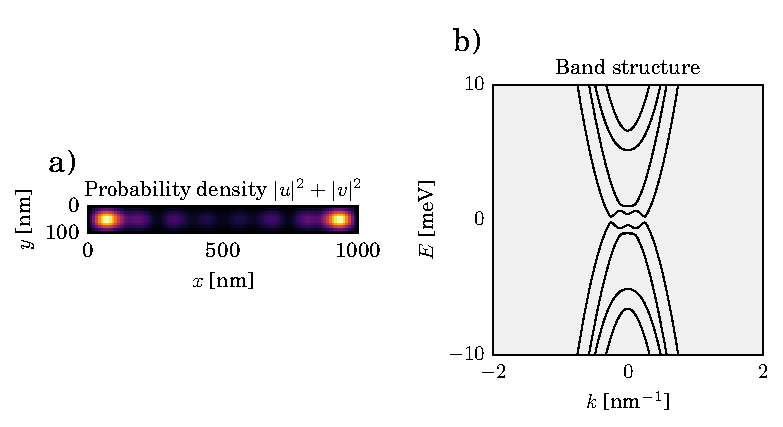
\includegraphics[width=0.95\textwidth]{chapter_introduction/figures/wavefunction_2d.pdf}
\par\end{centering}
\caption{Similar to Fig~\ref{fig:wavefunction_1d}, but for a 2D system.
\label{fig:wavefunction_2d}}
\end{figure}


\subsection{Phase diagrams}

We have seen that a topological band structure leads to Majoranas near the edges of the nanowire.
In the Hamiltonian (\ref{eq:rashba}) we see a few fundamental constants or constants that are material dependent.
However, the chemical potential $\mu$ and magnetic field $B$ can be adjusted in an experiment; asking for which values of $B$ and $\mu$ the system becomes topological is therefore a valid question.
In Fig.~\ref{fig:topo_bands} we see a phase diagram, which indicates for which value of $\left(B,\mu\right)$ the system is topological.
The color intensity indicates the size of the topological bandgap, which is a measure of the quality of the Majorana.
In chapter \ref{sec:phase-diagram} we explain how to calculate a phase diagram.

In the next chapter we will extend this model to three dimensions and add the orbital effect of the magnetic field.

\begin{figure}
\begin{centering}
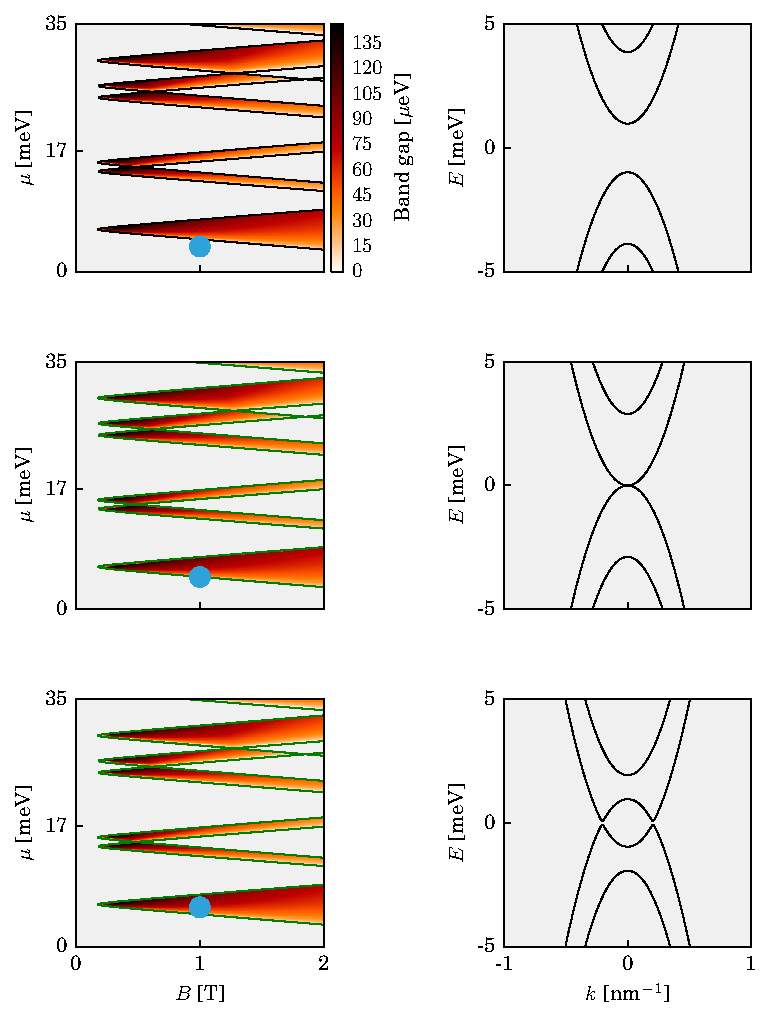
\includegraphics[width=0.8\textwidth]{chapter_introduction/figures/phase_diagrams_bands.pdf}
\par\end{centering}
\caption{Topological phase diagram of a 3D system.
On the left three phase diagrams with a blue dot that indicates the value of $B,\mu$ at which the band structure to the right of it is plotted.
The color in the phase diagrams depicts the topological region and its intensity the size of the topological gap.
The bottom band structure is topological, and a small gap is visible in the plot.
\label{fig:topo_bands}}
\end{figure}


\section{Structure of this thesis}

Here, we give a brief overview of the topics explored in the following chapters.
\vspace{1mm}

\subsection{Chapter~\ref{ch:introduction}: Introduction}
Abstract here for introduction
\vspace{1mm}

\subsection{Chapter~\ref{ch:adaptive}: Title here for adaptive}
Abstract here for adaptive
\vspace{1mm}

\subsection{Chapter~\ref{ch:orbitalfield}: Orbital effect of magnetic field on the Majorana phase diagram}
Studies of Majorana bound states in semiconducting nanowires frequently neglect the orbital effect of a magnetic field.
Systematically studying its role leads us to several conclusions for designing Majoranas in this system.
Specifically, we show that for experimentally relevant parameter values the orbital effect of a magnetic field has a stronger impact on the dispersion relation than the Zeeman effect.
While Majoranas do not require the presence of only one dispersion subband, we observe that the size of the Majoranas becomes unpractically large, and the band gap unpractically small, when more than one subband is filled.
Since the orbital effect of a magnetic field breaks several symmetries of the Hamiltonian, it leads to the appearance of large regions in parameter space with no band gap whenever the magnetic field is not aligned with the wire axis.
The reflection symmetry of the Hamiltonian with respect to the plane perpendicular to the wire axis guarantees that the wire stays gapped in the topologically nontrivial region as long as the field is aligned with the wire.
\vspace{1mm}

\subsection{Chapter~\ref{ch:supercurrent}: Supercurrent Interference in Few-Mode Nanowire Josephson Junctions}
Junctions created by coupling two superconductors via a semiconductor nanowire in the presence of high magnetic fields are the basis for the potential detection, fusion and braiding of Majorana bound states.
We study NbTiN/InSb nanowire/NbTiN Josephson junctions and find that the dependence of the critical current on the magnetic field exhibits gate-tunable nodes.
This is in contrast with a well-known Fraunhofer effect, under which critical current nodes form a regular pattern with a period fixed by the junction area.
Based on a realistic numerical model we conclude that the Zeeman effect induced by the magnetic field and the spin-orbit interaction in the nanowire are insufficient to explain the observed evolution of the Josephson effect.
We find the interference between the few occupied one-dimensional modes in the nanowire to be the dominant mechanism responsible for the critical current behavior.
We also report a strong  suppression of critical currents at finite magnetic fields that should be taken into account when designing circuits based on Majorana bound states.
\vspace{1mm}

\subsection{Chapter~\ref{ch:spinorbit}: Spin-Orbit Protection of Induced Superconductivity in Majorana Nanowires}
Spin-orbit interaction (SOI) plays a key role in creating Majorana zero modes in semiconductor nanowires proximity coupled to a superconductor.
We track the evolution of the induced superconducting gap in InSb nanowires coupled to a NbTiN superconductor in a large range of magnetic field strengths and orientations.
Based on realistic simulations of our devices, we reveal SOI with a strength of 0.15--0.35 eV\AA.
Our approach identifies the direction of the spin-orbit field, which is strongly affected by the superconductor geometry and electrostatic gates.
\vspace{1mm}

\subsection{Chapter~\ref{ch:zigzag}: Title here for zigzag}
Abstract here for zigzag
\vspace{1mm}

\subsection{Chapter~\ref{ch:shortjunction}: Robustness of Majorana bound states in the short-junction limit}
We study the effects of strong coupling between a superconductor and a semiconductor nanowire on the creation of the Majorana bound states, when the quasiparticle dwell time in the normal part of the nanowire is much shorter than the inverse superconducting gap.
This ``short-junction'' limit is relevant for the recent experiments using the epitaxially grown aluminum characterized by a transparent interface with the semiconductor and a small superconducting gap.
We find that the small superconducting gap does not have a strong detrimental effect on the Majorana properties.
Specifically, both the critical magnetic field required for creating a topological phase and the size of the Majorana bound states are independent of the superconducting gap.
The critical magnetic field scales with the wire cross section, while the relative importance of the orbital and Zeeman effects of the magnetic field is controlled by the material parameters only: $g$ factor, effective electron mass, and the semiconductor-superconductor interface transparency.

\subsection{Chapter~\ref{ch:weakantilocalization}: Title here for weakantilocalization}
Abstract here for weakantilocalization
\vspace{1mm}


\references{dissertation}
